\section{Methods}
As our project is to create a model with reinforcement learning, specifically DQN,
we do not have a predefined dataset. With this in mind, our methodology can be separated
into three parts.

\subsection{Reinforcement Learning}
Reinforcement Learning (RL) is a subset of Machine Learning (ML) where the
aim is to teach a model, called agent, via its interactions with the surrounding environment.
This method of learning requires no set of labeled or unlabeled data to be collected before
the learning actually starts. Instead the agent, typically a neural network,
is used for predicting the optimal action to be taken at each step based on its observation
and a reward is determined by the environment which is used for training the agent.
In RL, this environment is modeled as a Markov Decision Process (MDP)~\autocite{BUSONIU20188}.

\subsubsection{Markov Decision Process}
MDP is a mathematical framework based on Markov Chains for decision making processes
with inherent randomness. In Markov Decision Processes, we define:
\begin{itemize}
    \item \(S\): State Space (finite set),
    \item \(A\): Action Space (finite set),
    \item \(A_s\): Set of actions available at state \(s\),
    \item
          \(P^a_{ss'} = P_a(s,s') = P(s_{t+1} = s' \;|\; s_t = s, a_t = a)\) is the probability of action \(a\) in state \(s\) leading to state \(s'\),
    \item \(R_a(s, s')\): Reward received after transitioning from \(s\) to \(s'\).
\end{itemize}

\subsubsection{Markov Property}
For RL agents to work with MDPs we need the environment to be fully observable,
meaning that state \(s\) must capture all the characteristics of the environment.
In more technical terms, any state is \(S\) must satisfy the Markov Property which is defined as.
\begin{equation}
    P[s_{t+1} \;|\; s_t] = P[s_{t+1} \;|\; s_1, \ldots, s_t]
\end{equation}
This property essentially enables the environment to be memoryless which is required for
Markov Chains and more importantly its extension MDPs.

\subsubsection{Policy}
The objective in an MDP is to optimize the \textit{policy} of the decision making algorithm.
Here, we define the function \(\pi(s)\) that outputs the action chosen by the decision maker
based on the current state \(s\). This optimization mainly done by maximizing the cumulative
reward function. This function can be expressed as:
\begin{equation}
    G_t = \sum^{\infty}_{t=0}{\gamma^t R_a(s_t, s_{t+1})},\;
\end{equation}
where \(0\leq \gamma \leq 1\) is the discount factor. The equation above introduces the concept of \textit{discount factors}. This parameter is quite important as it is one of the hyperparameters of RL training loops. It is useful for avoiding cyclic behavior and infinite returns, and representing an exponentially increasing uncertainty for the future time steps.

Moreover, the policy that maximizes the function given above is regarded as as the
\textit{optimal policy} and denoted as \(\pi^*(s)\). It should be noted that this optimal policy is not necessarily unique.

\subsubsection{State-Value Function}
The state-value function, or just value function, is denoted by \(V_\pi(s)\). It is the expected return stating from state \(s\) and following policy \(\pi \) of an MDP\@. In most applications, it is used to evaluate how good being in a state is. It is mathematically expressed as:
\begin{equation}
    V_\pi(s) = E_\pi[G_t \;|\; s_t = s]
\end{equation}
As can be seen in the equation above, calculating the cumulative reward function is required
to find the value function of a state. This can be decomposed into a recursive function
as the current reward plus the discounted value function of the successor by utilizing
the Bellman Equation.
\begin{equation}
    V_\pi(s) = E_\pi[R_{t+1} + \gamma V_\pi(s_{t+1}) \;|\; s_t = s]
\end{equation}
With this done, we now define the state-value function that is produced by the optimal
policy \(\pi^*\) as the \textit{optimal state-value function}. In mathematical terms:
\begin{equation}
    V_*(s) = \max_\pi{V_\pi(s)}
\end{equation}

\subsubsection{Action Value Function}
The action value function, also called the Q-function, is the expected return starting from state \(s\), taking action \(a\), and then following policy \(\pi \). This is expressed as:
\begin{equation}
    Q_\pi(s,a) = E_\pi[G_t \;|\; s_t = s, a_t = a]
\end{equation}
Similar to the state-action function, we can also decompose this into a recursive function by redefining
\begin{equation}
    G_{t} = R_{t+1} + \gamma Q_\pi(s_{t+1}, a_{t+1}),
\end{equation}
and define the optimal action-value function as:
\begin{equation}
    Q_*(s,a) = \max_\pi{Q_\pi(s,a)}
\end{equation}

\subsubsection{Finding the Optimal Policy}
In all MDPs, three conditions are satisfied:
\begin{itemize}
    \item An optimal policy \(\pi^*\) exists (not necessarily unique),
    \item Optimal policy achieves the optimal state-value function
          \begin{equation}
              V_{\pi^*}(s) = V_*(s)
          \end{equation}
    \item Optimal policy achieves the optimal action-value function
          \begin{equation}
              Q_{\pi^*}(s,a) = Q_*(s, a)
          \end{equation}
\end{itemize}
These three assumptions can be used to shows that finding the optimal policy
\(\pi^*\) to solve the MDP can be done by maximizing over \(Q_*(s,a)\) with:
\begin{equation}
    \pi_*(a | s) =
    \begin{cases}
        1 & \text{if }\argmax_{a}{Q_*(s,a)} \\
        0 & \text{otherwise}
    \end{cases}
\end{equation}
This equation essentially means that finding the optimal policy can be done by
following the path given by \(Q_*(s,a)\) assuming that the optimal Q function is known~\autocite{mnih2013playing}.

\subsection{Neural Networks}
Artificial Neural Networks (ANNs), or simply Neural Networks (NNs), are
machine learning models that are loosely based on real life neurons and their connections.
Although the theoretical work for these types of models were mostly developed in mid
20\textsuperscript{th} century, the applications of them were quite limited considering
the computational power required for the necessary calculations.

\begin{figure}[h]
    \centering{}
    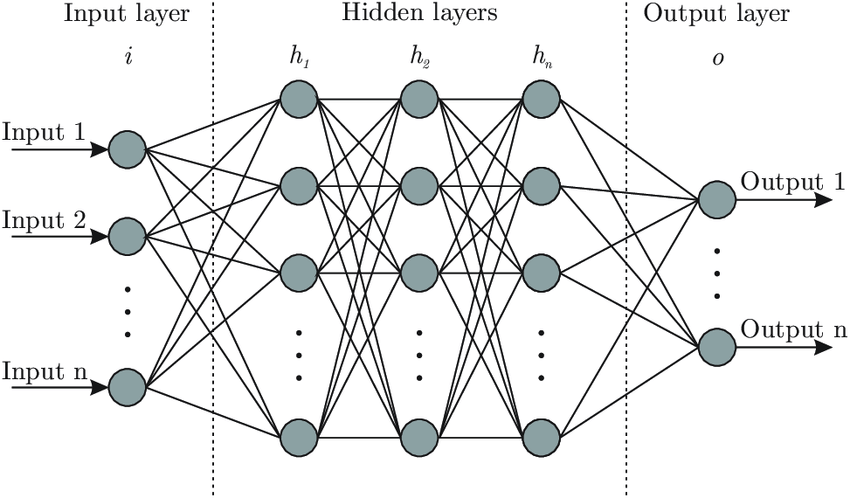
\includegraphics[width=\linewidth, height=0.3\textheight, keepaspectratio]{img/ann.png}
    \caption{A Basic ANN Structure~\autocite{buseyarentekin}}~\label{fig:ANN}
\end{figure}

In our project, the observation provided to the RL agent compromises of screenshots of
the game's graphics. Therefore, the NN we used is made up of mainly convolutional layers
for image processing with smaller fully connected layers at the end for decision making.
The entire neural network used is:
\begin{enumerate}
    \item Convolutional Layer: 32 filters,
    \item ReLu Activation Layer,
    \item Convolutional Layer: 64 filters,
    \item ReLu Activation Layer,
    \item Convolutional Layer: 64 filters,
    \item ReLu Activation Layer,
    \item Fully Connected Layer: 512 wide,
    \item ReLu Activation Layer,
    \item Fully Connected Layer: 3 wide
\end{enumerate}

\subsection{Deep Q Learning (DQN)}
The standard Q learning algorithm uses the training episodes to fill up a Q table where
each value corresponds to a specific action taken in a specific state. This method
functions properly when the amount of state action pairs are relatively low.
For example, the ``Cliff Walking Problem'', shown below, is simple enough that a Q table would be the feasible. In fact, the table would only have between 160 to 192 entries depending on  how the environment is defined.

\begin{figure}[h]
    \centering{}
    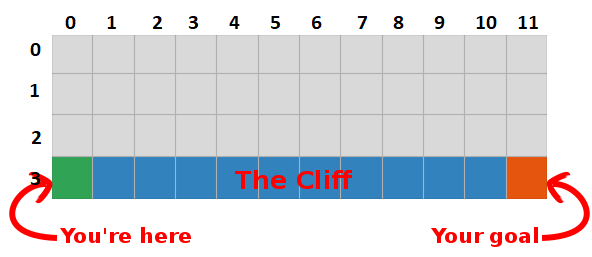
\includegraphics[width=\linewidth, height=0.3\textheight, keepaspectratio]{img/cliff_walking.png}
    \caption{Cliff Walking Problem~\autocite{Cliff_photo}}~\label{fig:CliffWalk}
\end{figure}


For more complicated environments, this approach quickly loses its feasibility.
In those cases, like what we have in Breakout, a neural network is used as a
nonlinear function approximator to replace the table. In DQN, the nn provides a
mapping from the give state \(s\), to the Q function of all possible actions in that
state \(Q(s,\underline{a})\).\\
The training loop of our network has a few additional, but still standard, features.
These are:
\begin{enumerate}
    \item
          \(\epsilon \)-greedy Policy: To simulate \textit{exploration}, the action will be chosen randomly with probability \(\epsilon \),
    \item Experience Replay Memory: To combat the unstable nature of deep reinforcement
          learning, a circular memory with a set size will be used to reduce the correlations
          between the sequence of observations used in every training batch.
    \item Target Network: An additional \textit{target network} is used to increase the
          stability of the learning.
\end{enumerate}
The final learning algorithm is given in~\autoref{algo:dqn} in~\autoref{app:dqn}.
